\documentclass[]{article}
\usepackage{amssymb}
\usepackage[backend=bibtex,style=authoryear,natbib=true]{biblatex} % Use the bibtex backend with the authoryear citation style (which resembles APA)

\addbibresource{example.bib} % The filename of the bibliography

\usepackage[autostyle=true]{csquotes} % Required to generate language-dependent quotes in the bibliography

\usepackage{tikz}
\usepackage{tikz-network}
\usepackage{breqn}

\usepackage{graphicx}
\usepackage{subcaption}
\usepackage{multirow}
\usetikzlibrary{fit}
\usetikzlibrary {arrows.meta,graphs,shapes.misc}
\usetikzlibrary {positioning}

\newcommand{\bn}{\textbf{n}}
\newcommand{\tabhead}[1]{\textbf{#1}}

\begin{document}

Intrinsic image model was introduced by \cite{intrinsic-image}. It represents that an image $ I $ can be decomposed as the element-wise product between the reflectance $ R $ of the object and the shading $ S $ produced by the interaction between light and objects.
\[ I =R  \odot S\]
The equation can be further decomposed based on different surface models. If assume the object surfaces are Lambertian surfaces, i.e. the diffuse surfaces, the equation can be decomposed further as follows
\[ I = \rho  \odot (L_0 \textbf{L} \cdot  \textbf{N}) \]
where $ \rho $ is the reflectance of diffuse surface, also know as albedo, $ L_0 $ is the radiance of  incoming light, i.e. irradiance, $ \textbf{L} $ is the direction of incoming light as unit vector map and $ \textbf{N} $ is the surface normal also as unit vector map.

The decomposition gives a constraint of the normal map with given other information, which can be considered further in the deep learning model. The image $ I $ is given in the RGB-D image, the light map $ \textbf{L} $ can be calculated based on the light source and the vertex map. 

L->L0L 



\newpage 
 As shown in Figure \ref{fig:lambertian-surface}, 
\begin{figure}[th]
	\centering
	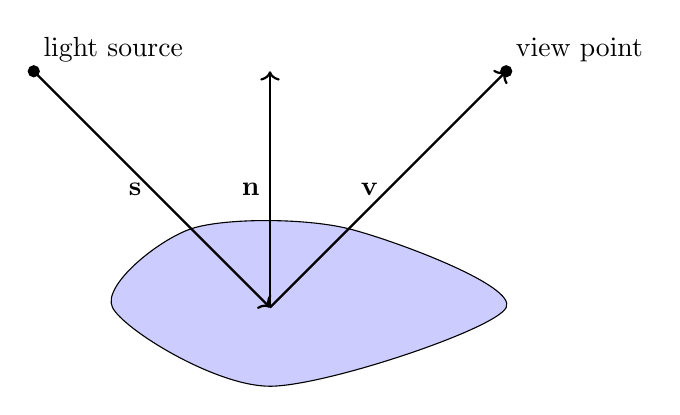
\begin{tikzpicture} 
		% reference lines
		\draw [fill=blue!20] plot [smooth cycle] coordinates {(0,0) (1,1) (3,1) (5,0) (2,-1)}; %% surface element
		\draw[thick, ->] (2,0) -- (2,3) node[midway, left] {$ \textbf{n} $}; %% normal
		\draw[thick, ->] (-1,3) -- (2,0) node[midway, left] {$ \textbf{s} $}; %% source direction
		\draw[thick, ->] (2,0) -- (5,3) node[midway, left] {$ \textbf{v} $}; %% view direction
		\filldraw[black] (-1,3) circle (2pt) node[anchor=south west]{light source}; %% light source
		\filldraw[black] (5,3) circle (2pt) node[anchor=south west]{view point}; %% view point		
	\end{tikzpicture}	
	\caption{Lambertian Surface}
	\label{fig:lambertian-surface}
\end{figure}
According to the Lambertian reflectance model, the relationship between image and the surface model is 
\[ I = \rho (\textbf{N} \cdot \textbf{L}) \]

where $ I $ is the total power , $ \rho $ is the albedo,  $ N $ is the normal map and $ L $ is the incoming light direction.

\end{document}
